\label{}
\section{Background and Context}
\textit{This section creates the background and describes the context of the project to ensure the problem formulation refers to real-life scenarios and challenges of actuality.}\\

The characteristic of today's mobile robots most sought after is autonomy. This demand has evolved from very early technologies started by the first industrial revolution, Industry 1.0. It is because of these beginnings that robots are rather designed for manufacturing than other fields. \\

Industry 1.0 is referred to as the 'Golden Age' of productivity started by the industry's mechanisation using non-electricity powered technologies such as the steam engine, motorised machines, etc. These new levels of automation lowered production costs and brought economic and social development \cite{uk}.\\


Industry 2.0 is marked by the need of mass-production. Electricity-based technologies were introduced in the industry such as assembly lines, automated machines, etc. Automation meant that products' quality could be guaranteed. As such manufacturing processes started to involve practices of standardization. Needless to say, these technological evolution spurred development in other areas such as computing and communication technologies. \cite{uk}\\


\begin{figure}[H]
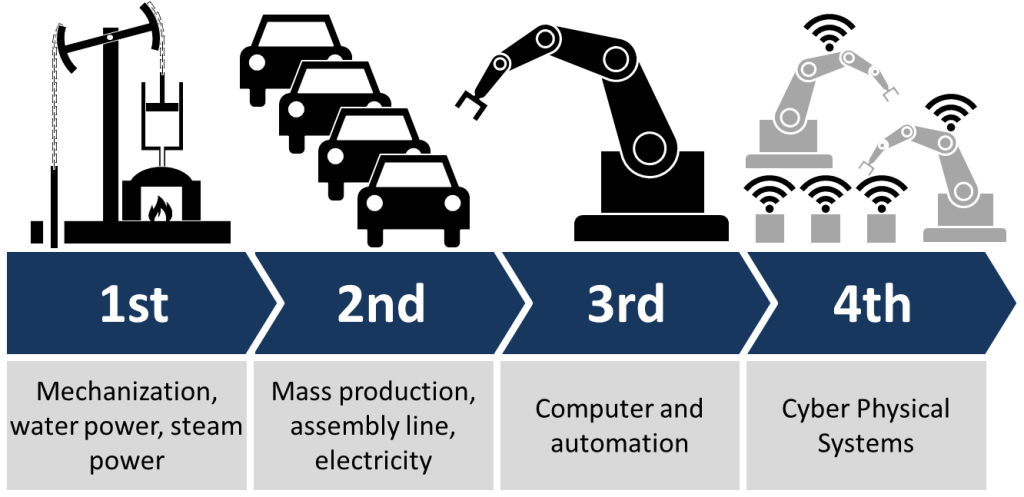
\includegraphics[scale=0.4]{Figures/industry4.png}
\centering
\caption{The delimination of the four major industrial revolutions. The classification of technologies under each revolution is generally not the same throughout the community. Source: \cite{site}.}
\label{industry4}
\end{figure}


Cross-disciplinary technologies such as mechatronics, robotics and autonomous systems mark the start of Industry 3.0 - the digital manufacturing. Combining digital innovations and connectivity, manufacturing processes become partially or fully digitized for better resource management and responsiveness to customer's demands. Robots advance from doing highly-repetitive tasks to being involved in series of tasks with a certain underlying level of complexity. Robots become smarter, faster and cheaper. \cite{uk}\\

As the technological development brought paradigm shifts leading to industrial revolutions \cite{industry4}, the forth industrial revolution brings advanced digitalisation of so many more domains than the industry, that Industry 4.0 refers strictly to related concepts such as: smart factory, smart manufacturing, industrial internet-of-things (IOT), embedded systems, harnessing the potential of connected devices, communicating with each other to make reliable decisions. \cite{uk} This is also depicted in Figure \ref{industry4} as cyber-physical systems. \\

Cyber-physical systems refer to the merge between the real, physical world and the digital \cite{industry4}. The reliability of these machines has led to minimal human intervention if not at all. As the robots became smarter, the tasks solved are increasingly more complex. Examples of such task are collaborative robots (human-robot close interaction), robots finishing manufacturing processes with no human intervention, real-time deliveries of materials by autonomous mobile robots, etc.\\

The interconnection of all devices (sensors, machines, robots, tools) allows for data gathering, exploration and fusion for better decisions. Based on these data a plethora of technologies can be employed in a smart factory. Some of the most important technologies defining Industry4.0 can be visualized in Figure \ref{industry40} with autonomous robots as the driver for technologies that can further improve their capabilities.

\begin{figure}[H]
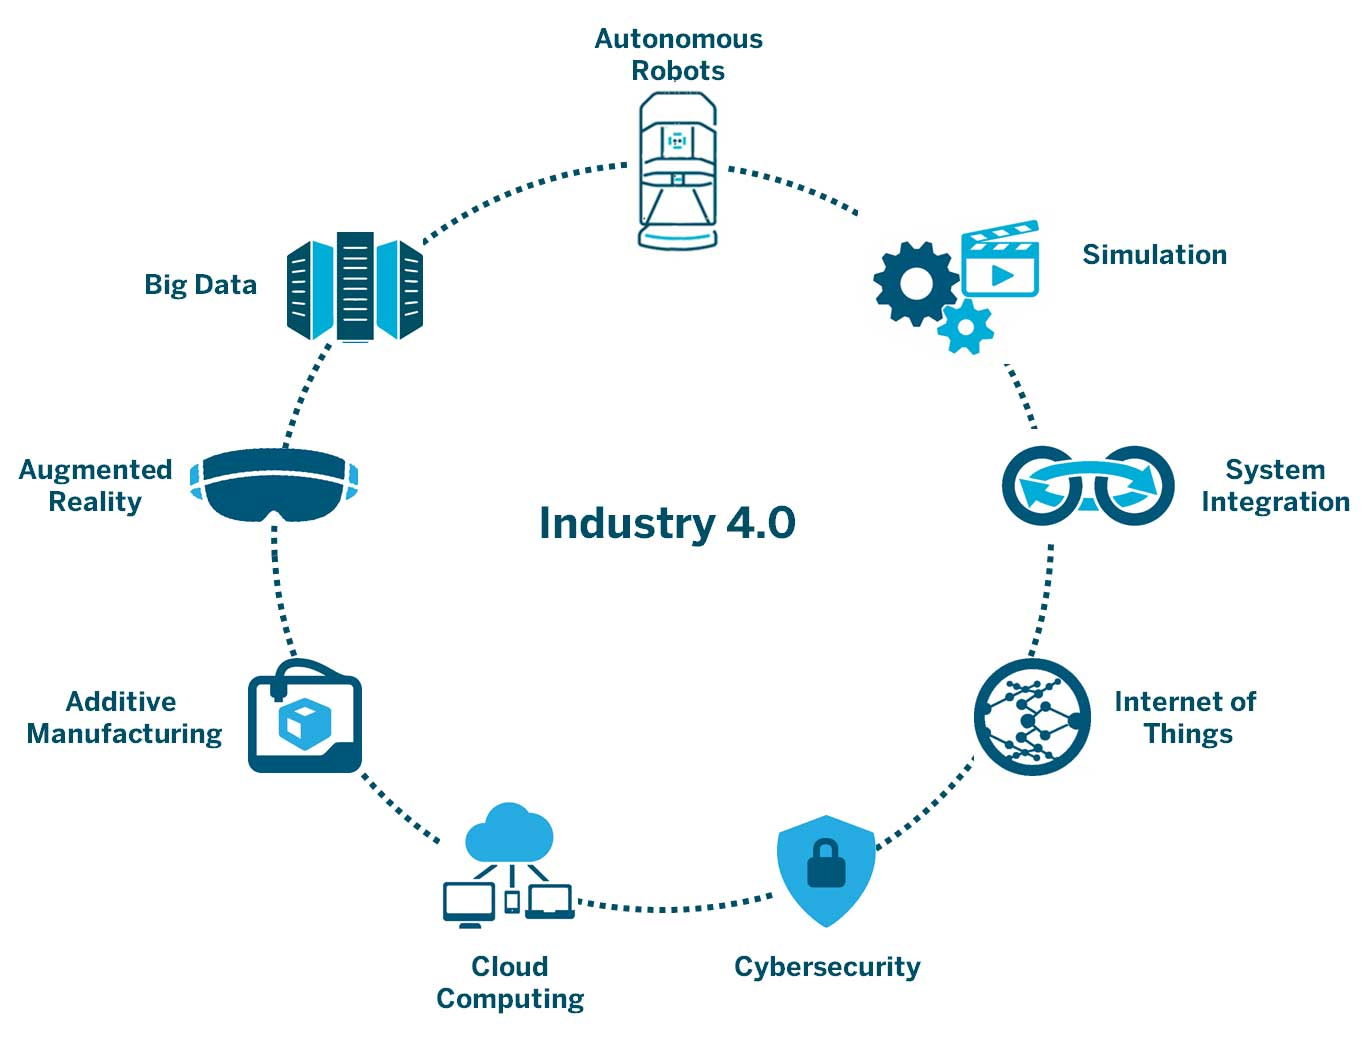
\includegraphics[scale=0.3]{Figures/Industry40.jpg}
\centering
\caption{The key technologies of the Industry 4.0 that are used in a smart factory \cite{boston}. Source: \cite{aethon}}.
\label{industry40}
\end{figure}

Autonomous robots are an important example for countless industries, especially for industrial manufacturing context. Autonomous robots needed in manufacturing are of many types (manipulators, machines, mobile) but of relevance for this project remain the mobile robots. Their role in the smart factory can be diverse but of importance remains the ability to autonomously navigate from point-to-point the factory's floors avoiding obstacles or other mobile robots, and eventually, carry materials needed in other parts of the plant. Such robots can be integrated in a manufacturing execution systems and receive signals as to where and when to move and what orientation to have. As exemplified in \cite{aethon}, modular conveyor belts can be placed on mobile robots and depending on the production needs, these robots can redesign the manufacturing flow near designated programmable logic controllers (PLCs) \footnote{PLC is an industrial computer designed to control manufacturing processes such as assembly lines, robotic tools, etc.}.\\

Mobile robots for industrial manufacturing have not always been completely autonomous, but to varying degrees. An autonomous mobile robot can make decisions on how to get from point A to point B. Complete autonomy of the mobile robot is of interest for this project and it is discussed further in the next section.


\section{Project Objective}

\textit{This section presents the objective of the project and the connection to the real-world problem it tries to solve.}\\

 A prevailing type of robots in industrial manufacturing are the automated guided vehicles (AGV) defined by a mobile robot following a magnetic or painted path \cite{agv}. The robot only needs to know the distance along the pathway to the target not its location. Obstacles on the pathway are avoided by the use of LiDar. Being limited by their wired pathway, the AGV are inflexible and cannot leave the physical path.\\
 
 It is possible, however, if there exists a virtual map of the working environment the robot may be able to follow a virtual pathway using the map and knowing there it is on the map with the help of special reflective marks. The robot is using a LiDar and triangulation with multiple marks to calculate its position. This is shown in the figure below (Figure \ref{agv}).
 
 \begin{figure}[H]
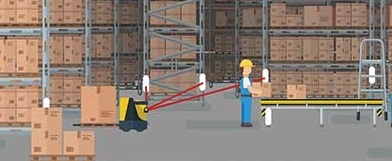
\includegraphics[scale=1.5]{Figures/agv1.jpg}
\centering
\caption{Industrial mobile robot using a map of the environment known apriori to move and locate on it. The positioning is done with the help of reflective markers strategically placed in the environment \cite{agv}. Source: \cite{agv}}.
\label{agv}
\end{figure}

A disadvantage for this type of autonomy are the placement of the reflective markers which have to be detected by the LiDar. As such the markers have to be placed at the same height of the sensor. Moreover, problems arise from the obstruction of markers by high shelves, moving objects or people standing in front of one. Since for an accurate localization, the robot needs at a minimum 3 markers, the chances of detecting 3 unobstructed markers drop with an increasing busy industrial environment.\\

Autonomous mobile robots (AMR) are defined as the robots free of any enhanced-infrastructure for navigation \cite{agv}. These robots are flexible as can travel anywhere in the industrial environment while avoiding obstacles and humans in their path. The map of the environment is not known apriori. The main sensor used is still the LiDar. In order to operate in such busy environments fully autonomously the robots needs to create a map of the environment while finding its position on the map and taking decisions on reaching from point A to point B. Path planning and tracking needs to consider obstacle avoidance as an important dimension of AMRs especially when working near humans.\\

An AMR needs to create a map of an unknown environment while finding its own position on the map. In order to solve this problem it uses an algorithm. Simultaneous Mapping and Localization (SLAM) is a solution to the navigation problem of a robot in an unknown environment. It tries to answer two questions: where am I? and how does the environment look like? It is simultaneous because it solves what metaphorically is a chicken-and-egg problem: the robot needs a map to know where it is however to create a map it needs to know where it is located.\\

SLAM is a key component in autonomous mobile robots. Using relative observations of the surroundings the platform can navigate in an unknown environment while creating a map. Multiple sensors can be used with SLAM with the most prevalent: odometer and LiDar however local positioning system can also be used. Each sensor used has an algorithm to determine the robot's motion or position. \cite{agv}. Hence, SLAM is rather a methodology for sensor fusion that solves the navigation problem in an unknown environment having constraints on the resources available: sensors, storage, computational capacity and complexity, algorithm robustness.\\

As an algorithm, SLAM is comprised of two parts: robot localization and building of the map. Robot state is what builds the localization part being comprised of simple instances: position, orientation, velocity, etc. while mapping is a representation of landmarks position, obstacles, features, etc. A map is needed to reduce the position error of the robot and to allow for a visualized path planning and tracking by an operator \cite{past}. In the absence of a map, the robot depends on dead-reckoning \footnote{Dead-reckoning is a process of finding current position based on the previous position plus measured distance elapsed on the course. It accumulates directional errors making the robot drift from the set course. The accuracy of this methods can be improved by adding positional sensors such as GPS/absolute positional system.} which leads to an accumulation of error and the robot drifts from the set position. Hence both parts have to be solved simultaneously. \\

\subsubsection{Specific Context}

The context of this project is to develop a low-cost mobile robotic solution to work in a smart production laboratory. It is envisioned that the mobile robot to be an integrated part of a smart production line receiving jobs from a delegating server to transport for example Lego bricks. There are designated dropping stations where the robot has to arrive, receive the packet, receive the location of the new delivery station and arrive at the specified delivery station. An illustrative example of the laboratory environment can be seen in Figure \ref{figure:lab}. 

 \begin{figure}[H]
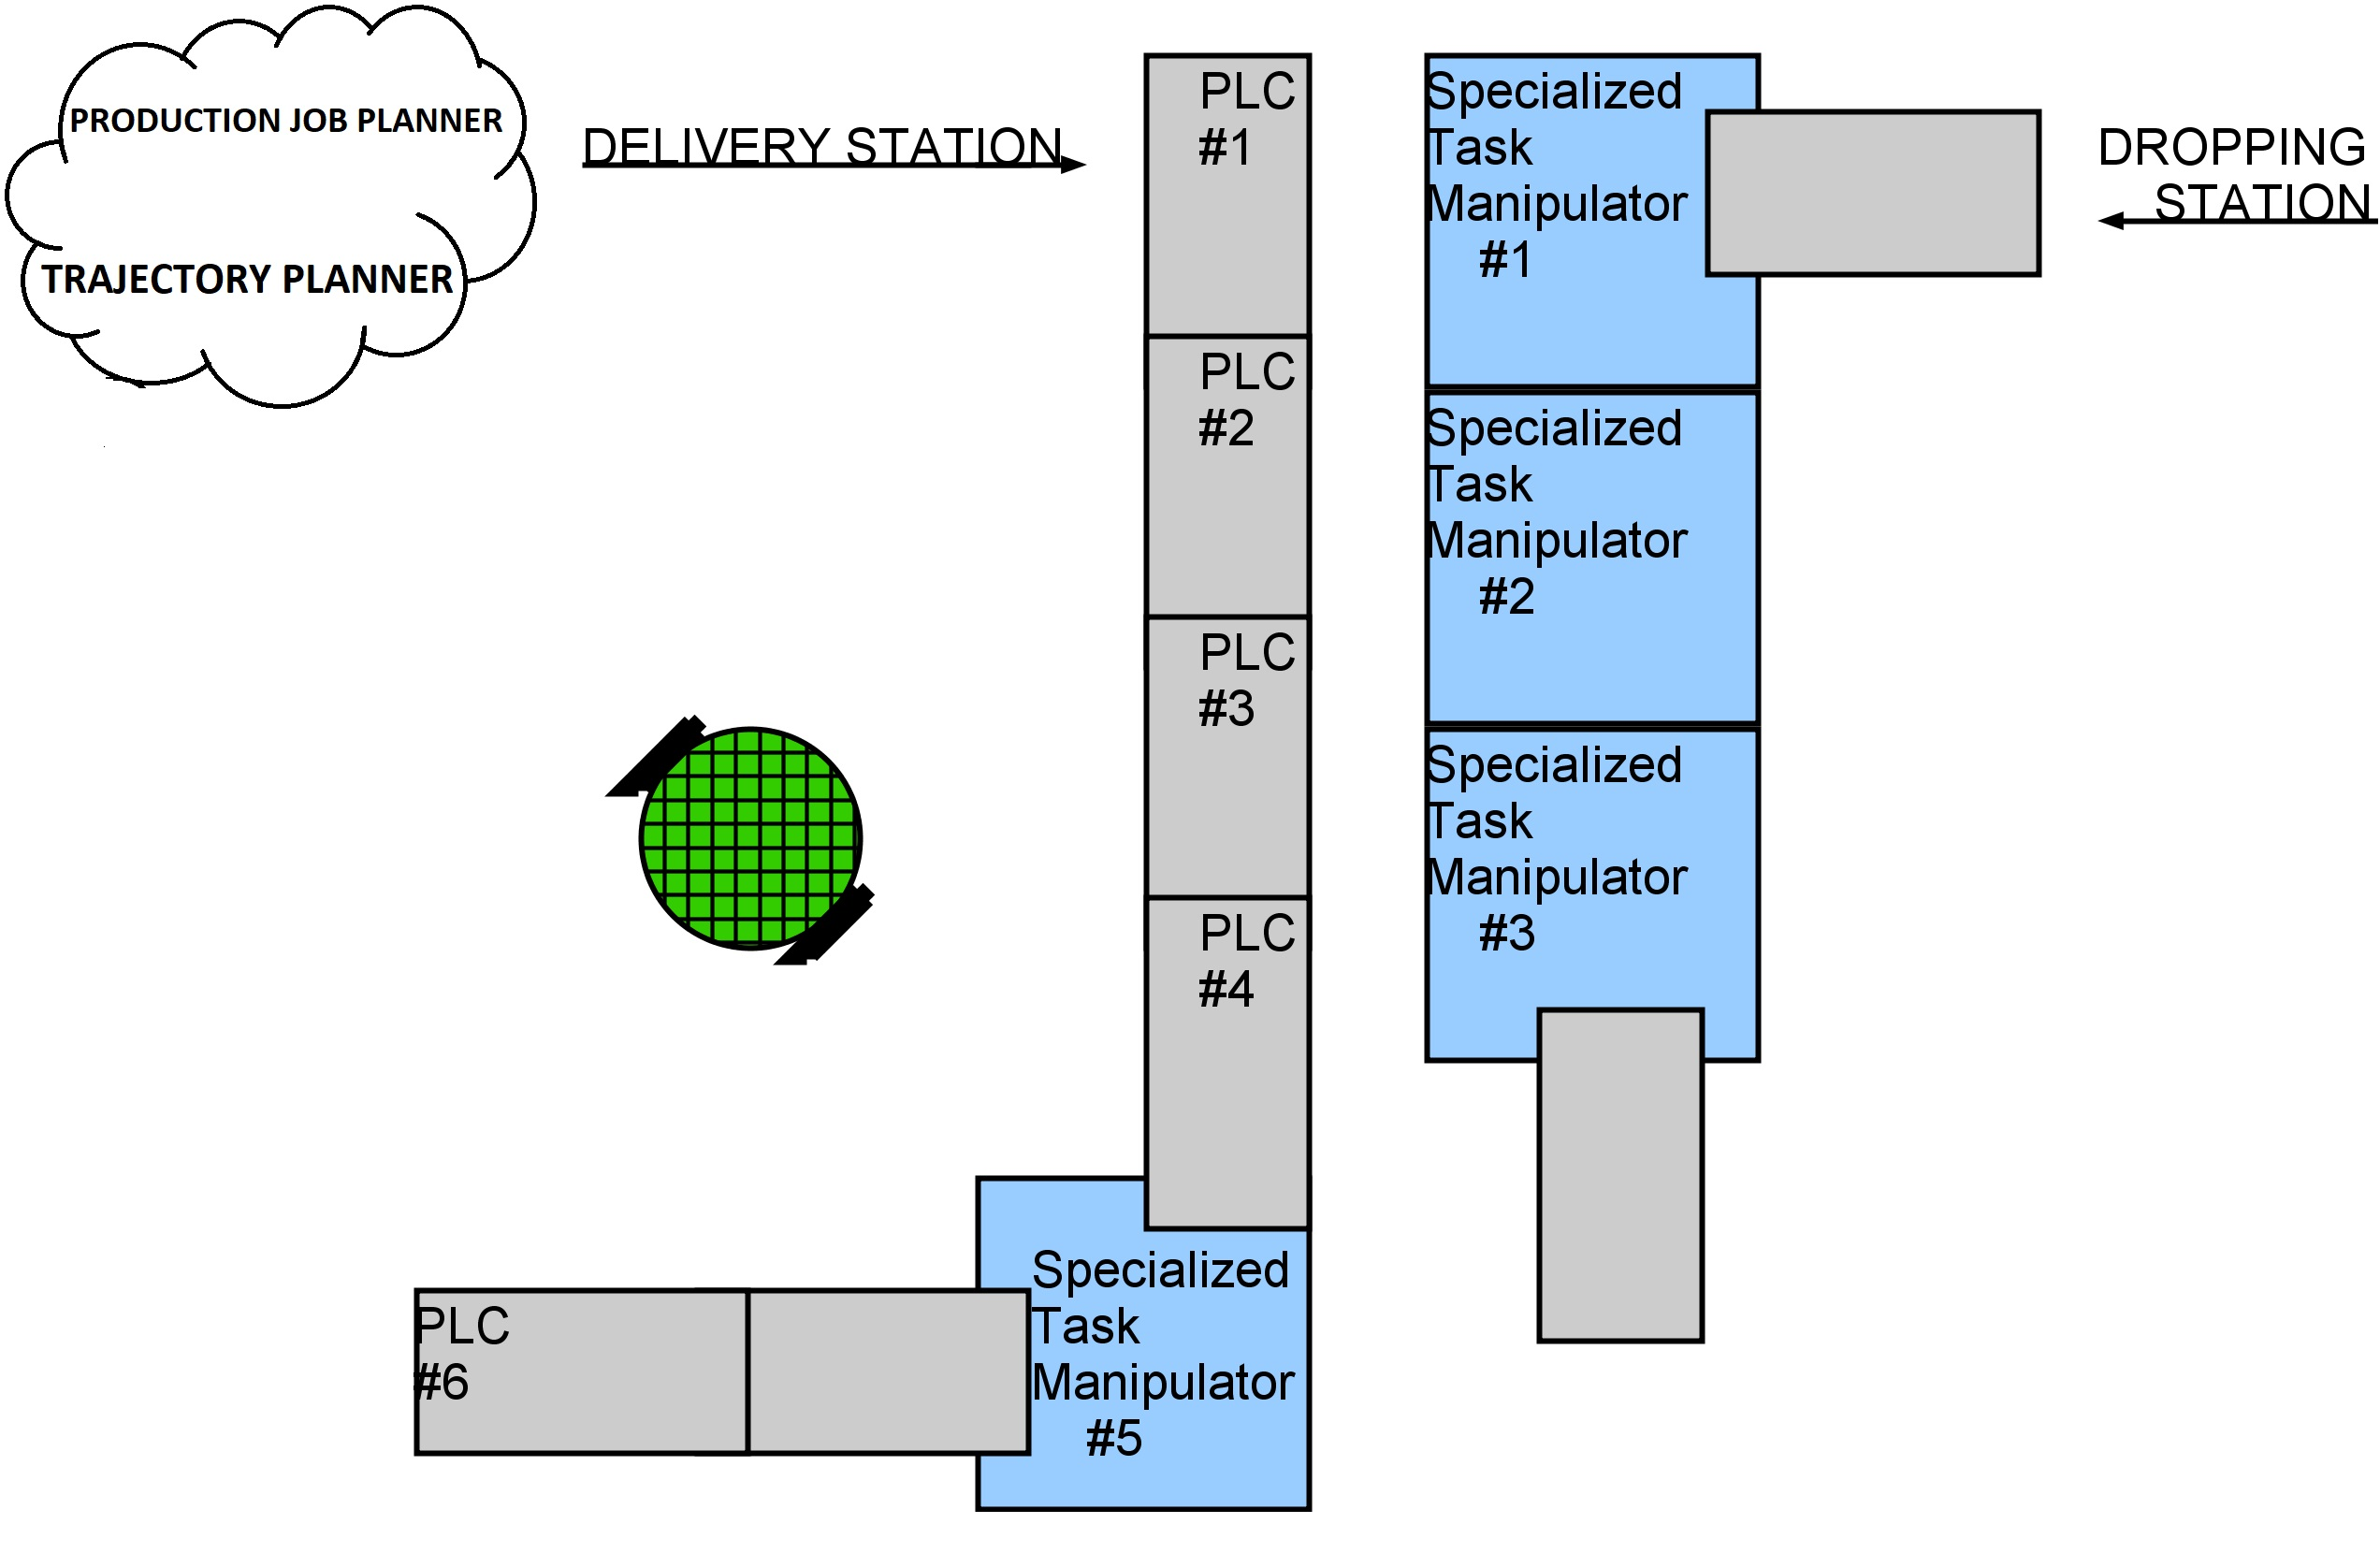
\includegraphics[scale=0.25]{Figures/plc_production line_cloud.jpg}
\centering
\caption{Illustrative example of the Smart Production Lab at Aalborg University. It can be seen different production units - PLCs in gray and robot manipulators for specialized tasks in blue with designated dropping and delivery stations for the mobile robot }.
\label{figure:lab}
\end{figure}

In the specific context of the Smart Production Lab, each production unit involved - PLCs, manipulators, collaborative robots, etc. has an unique id and task assigned by the production planner. The mobile robot is also part of the production line and receives an id and a task from the server - which is on a cloud. As a job is received, the trajectory planner calculates the route of between the current position of the robot and the desired location. The trajectory planner communicates where the robot should go and the robot communicates back the current location on the map.\\

The map of the environment is unknown (landmarks/obstacles are not known) as it is expected not all operators to have or be able to produce a map of the production environment. The robot is equipped with the standard sensors for performing SLAM - magnetometer, encoders and LiDar. There is also a low-cost ultrasonic solution for local positioning of the robot to be used in the algorithm to improve robot's pose in the map. Navigation or planning of the trajectories of the robot is done at the higher level of the delegating server. \\

The SLAM algorithm is the solution to estimate the robot's current position based on low-cost and noisy sensors, while not having a map of the environment or a high-precision localization sensor to be used as ground-truth. 
In a typical implementation of the SLAM algorithm, the Kalman filter is used for sensor fusion of positional data. Other flavours of the Kalman filter can also be used, as well as the particle filter. It depends as said before on the resources available. Regarding SLAM as a methodology for creating navigation solutions dependent on the environment, it means that there are many types of SLAM methods with different features depending on the surroundings of the robot, robot resources and requirements. Four approaches to SLAM implementation can be seen in Figure \ref{slam} where depending on the resources available one or two approaches can be implemented.

 \begin{figure}[H]
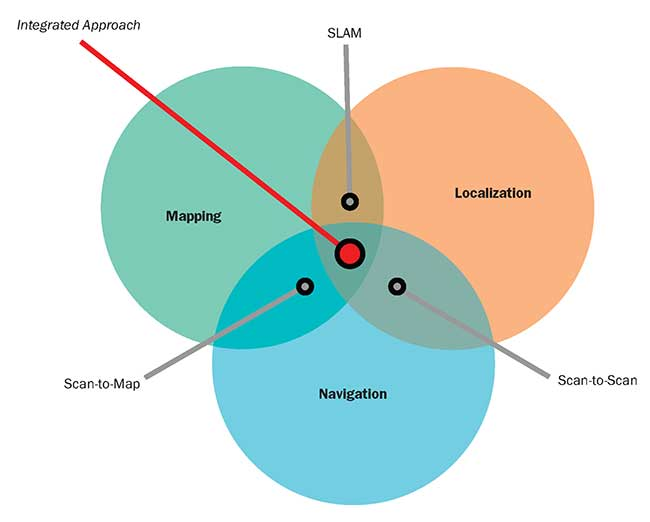
\includegraphics[scale=0.5]{Figures/slam.jpg}
\centering
\caption{The four types of approaches to localization, mapping and navigation. Source: \cite{agv}}.
\label{slam}
\end{figure}

\subsubsection{Scan-to-Scan}
This method does not require a map as can be seen from Figure \ref{slam} but it can estimate the robot's position and pose from sequential LiDar data. The position estimate is updated continuously and is subject to drift in long-term use. It is used for process startup when a map is not yet created or when the environment has changed \cite{agv}.\\

\subsubsection{Scan-to-Map}
The algorithm requires a stored map of the environment while the robot estimates its position by matching actual readings to the map. The matching can give erroneous results if the environment is symmetric or similar in different regions and if the stored map does not match the readings.\\

\subsubsection{Integrated Approach - full SLAM}
This algorithm solves all three aspects of the mobile robot: localization, mapping and navigation. It can be done by adding more sensors such as a camera to help extract environment features and match object in a map better, but at the expense of computational power.\\

While each algorithm presented has both advantages and disadvantages, a combination of at least two is used to reach the requirement specifications for the mobile robot. Next section actually formulates the problem statement of the project and the methodology of how it intends to solve it.\\ 




